\documentclass{article}

% if you need to pass options to natbib, use, e.g.:
%     \PassOptionsToPackage{numbers, compress}{natbib}
% before loading neurips_2026

% The authors should use one of these tracks.
% Before accepting by the NeurIPS conference, select one of the options below.
% 0. "default" for submission
\usepackage[preprint]{neurips_2026}
% the "default" option is equal to the "main" option, which is used for the Main Track with double-blind reviewing.
% 1. "main" option is used for the Main Track
%  \usepackage[main]{neurips_2026}
% 2. "position" option is used for the Position Paper Track
%  \usepackage[position]{neurips_2026}
% 3. "eandd" option is used for the Evaluations & Datasets Track
 % \usepackage[eandd]{neurips_2026}
 % if you want to opt-in for a de-anomymized submission (not recommended, but OK):
 %\usepackage[eandd, nonanonymous]{neurips_2026}
% 4. "creativeai" option is used for the Creative AI Track
%  \usepackage[creativeai]{neurips_2026}
% 5. "sglblindworkshop" option is used for the Workshop with single-blind reviewing
 % \usepackage[sglblindworkshop]{neurips_2026}
% 6. "dblblindworkshop" option is used for the Workshop with double-blind reviewing
%  \usepackage[dblblindworkshop]{neurips_2026}

% After being accepted, the authors should add "final" behind the track to compile a camera-ready version.
% 1. Main Track
 % \usepackage[main, final]{neurips_2026}
% 2. Position Paper Track
%  \usepackage[position, final]{neurips_2026}
% 3. Evaluations & Datasets Track
 % \usepackage[eandd, final]{neurips_2026}
% 4. Creative AI Track
%  \usepackage[creativeai, final]{neurips_2026}
% 5. Workshop with single-blind reviewing
%  \usepackage[sglblindworkshop, final]{neurips_2026}
% 6. Workshop with double-blind reviewing
%  \usepackage[dblblindworkshop, final]{neurips_2026}
% Note. For the workshop paper template, both \title{} and \workshoptitle{} are required, with the former indicating the paper title shown in the title and the latter indicating the workshop title displayed in the footnote.
% For workshops (5., 6.), the authors should add the name of the workshop, "\workshoptitle" command is used to set the workshop title.
% \workshoptitle{WORKSHOP TITLE}

% "preprint" option is used for arXiv or other preprint submissions
 % \usepackage[preprint]{neurips_2026}

% to avoid loading the natbib package, add option nonatbib:
%    \usepackage[nonatbib]{neurips_2026}

\usepackage[utf8]{inputenc} % allow utf-8 input
\usepackage[T1]{fontenc}    % use 8-bit T1 fonts
\usepackage{hyperref}       % hyperlinks
\usepackage{url}            % simple URL typesetting
\usepackage{booktabs}       % professional-quality tables
\usepackage{amsfonts}       % blackboard math symbols
\usepackage{nicefrac}       % compact symbols for 1/2, etc.
\usepackage{microtype}      % microtypography
\usepackage{xcolor}         % colors
\usepackage{graphicx}
\usepackage{comment}
\usepackage{float}
\usepackage{enumitem}


% Note. For the workshop paper template, both \title{} and \workshoptitle{} are required, with the former indicating the paper title shown in the title and the latter indicating the workshop title displayed in the footnote. 
\title{Junkyard Autograder Benchmarking \\ \large Project Specification}



% The \author macro works with any number of authors. There are two commands
% used to separate the names and addresses of multiple authors: \And and \AND.
%
% Using \And between authors leaves it to LaTeX to determine where to break the
% lines. Using \AND forces a line break at that point. So, if LaTeX puts 3 of 4
% authors names on the first line, and the last on the second line, try using
% \AND instead of \And before the third author name.


\author{
  Abas Mohamed \\
  \texttt{aam037@ucsd.edu} \\
  \And
  Ayushmaan Puri \\
  \texttt{aypuri@ucsd.edu} \\
  \And
  Richard Vo \\
  \texttt{rivo@ucsd.edu} \\
  \And
  Tom Zhang \\
  \texttt{shz078@ucsd.edu} \\
}

% Mentors, may have to include for secondary authors
% \author{
%   Christopher Crutchfield \\
%   \texttt{ccrutchf@ucsd.edu} \\
%   \And
%   Raymond Dueñas \\
%   \texttt{r1duenas@ucsd.edu} \\
%   \And
%   Alexander Redding \\
%   \texttt{alredding@ucsd.edu} \\
% }


\begin{document}


\maketitle


\begin{abstract}
The Junkyard project aims to repurpose old and unusable smartphones as valuable compute units for distributed computing. One of these applications is for a class of students testing their code for timing and accuracy. In the most recent offering of CSE 160, the class was allocated 40 reservable GTX 1080 Ti pods on DSMLP\footnote{UCSD's Data Science and Machine Learning Platform} shared across roughly 330 students. Demand routinely exceeded supply around assignment deadlines, creating bottlenecks that delayed feedback and frustrated students. Student submissions don't need raw GPU power, they need a consistently available and standardized execution environment. A cluster of repurposed smartphones can provide exactly that, at a fraction of the cost and with hardware that would otherwise be discarded. Smartphones are particularly well-suited for this use case: they are power-efficient, self-contained compute nodes with standardized hardware profiles, and their ubiquity means institutions can source them at little to no cost. Rather than competing for shared high-performance resources, students would submit to a dedicated phone cluster optimized specifically for lightweight, reproducible execution. This project investigates two core questions. First, how many phones are needed to serve a class of n students without meaningful queuing delays? Second, what is the throughput ceiling of a phone cluster, measured in submissions per unit time, before the system degrades under load?
\end{abstract}



\section{Project Charter}


\subsection{Approach}
The results of previous work have shown the effectiveness of tools (e.g. autograders), that provide immediate feedback on assignments given to students [1-3]. In particular, Mitra [2] concluded that feedback from an autograder helped students improve their ability to write better code consistent with specifications. Sherman et al. [1] found that student submission rates are higher when submitted on an autograder instead of through a manually graded platform. However, McBroom et al. [4] saw non-homogeneous student submission trends. Hence, in order to accurately estimate the number of phones needed in a class of n students, we must take into account these class-specific details.

More specifically, we need student submission trends and the exact load that is put upon DSMLP throughout the lifetime of a programming assignment. The anonymized student data would consist of: student submission runtime, submission trend, and pod usage.

Subsequently, we can build a model from the collected data and then randomly sample from the model to represent “mock” student submissions. We decided on the Gaussian mixture model, using the sklearn.mixture module. The submission trends of students who submit early can be viewed as a Gaussian distribution unique from the trends of those who submit near the deadline. In that sense, our model would be a mixture of these Gaussian distributions of  different student submission behavior.

Following our data generation, we will build a simulator that can take the mock submissions and simulate the necessary load required to run each submission. The simulator should support variable simulation speeds to save time in comparison to running real submissions on the clusters. Although the simulator would work standalone on anyone’s personal computer, the simulator should still be able to distribute tasks to the phone autograder.

The virtual simulator will need to be calibrated to the true latency and throughput of the Qualcomm and Pixel clusters to accurately represent it at scale. We will accomplish this by initially running submissions on our currently available $\sim$ 20 clusters to get key parameters, such as delays in communication, scheduling latency, physical limitations of ram and thermals, actual job performance data, and finally job exit codes. This will allow us to continue with the next phase of gathering key metrics from our simulated clusters which should mirror the increased number of incoming physical clusters. 

\begin{comment}
\begin{figure}
  \centering
  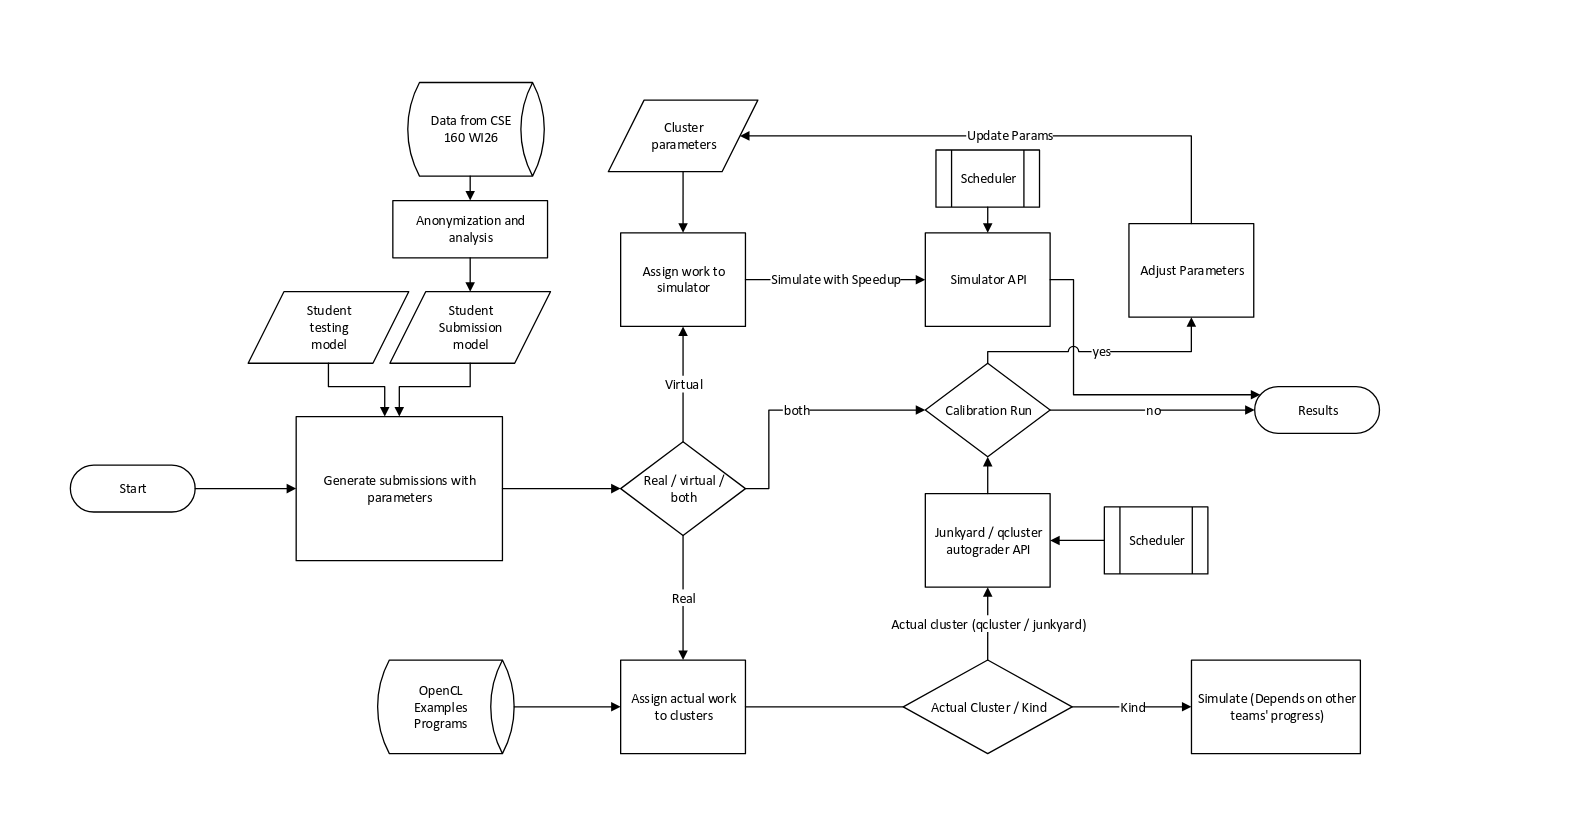
\includegraphics[scale=0.75, width=\linewidth]{images/workflow.png}
  \caption{Project workflow.}
\end{figure}
\end{comment}

\begin{figure}
  \centering
\makebox[\textwidth]{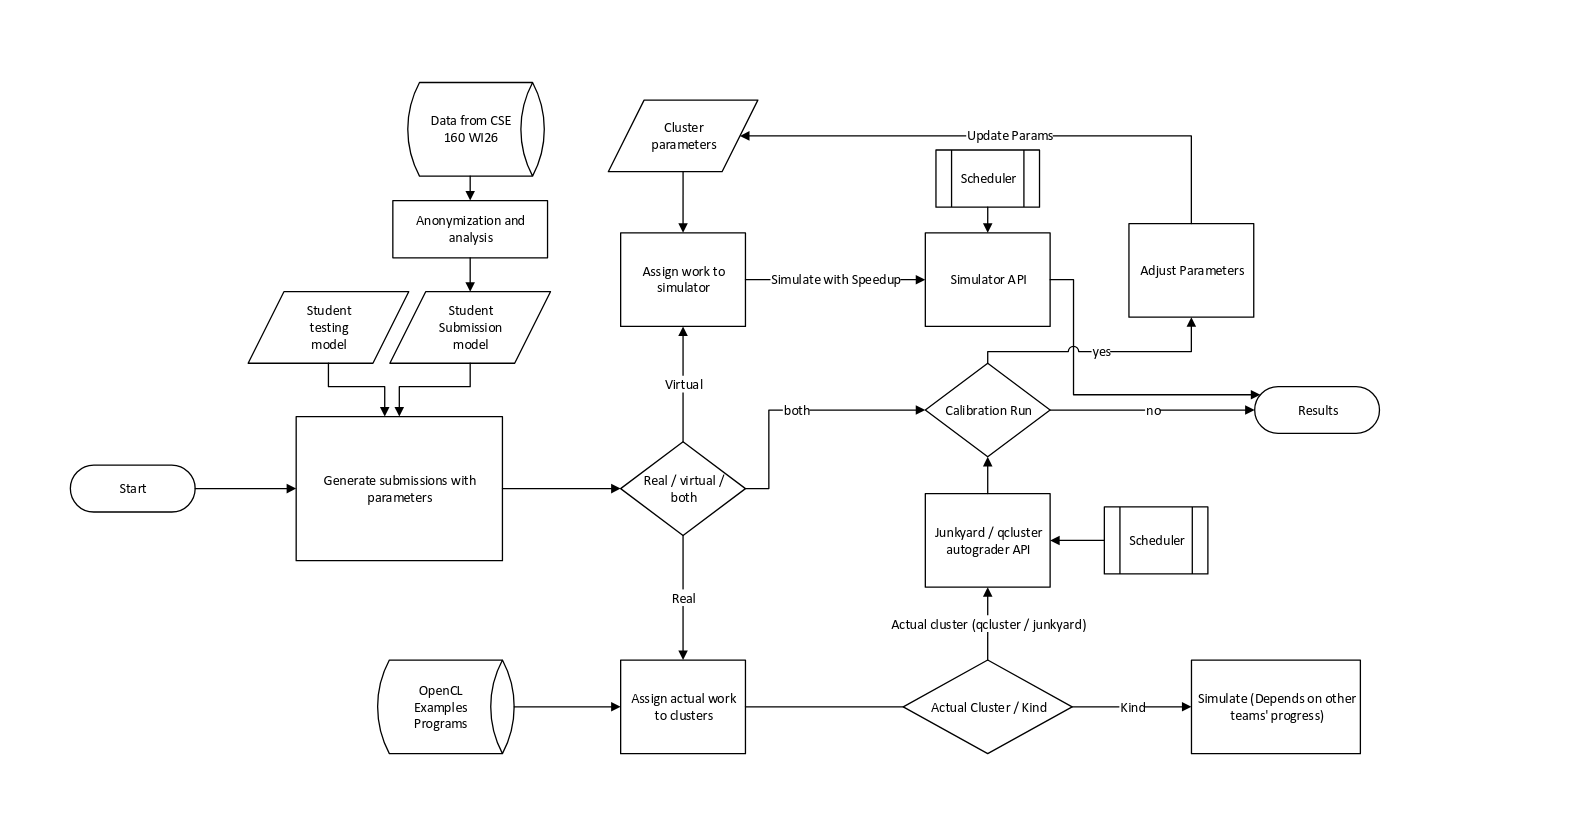
\includegraphics[width=1.65\textwidth]{images/workflow.png}}
\caption{Project workflow.}
\end{figure}


\subsection{Constraints, Risk, and Feasibility}


Our initial constraint is with data collection for student submissions. We currently have historical data of CSE 160: Introduction to Parallel Programming in Winter 2026 for both the Qualcomm Cluster and the Junkyard Cluster. However, this data is not consolidated on the autograder platform – Gradescope. Thus, the only feasible option is to web scrape the data ourselves. Furthermore, student submissions and grades are protected under FERPA and cannot be accessed by people outside of instructors of that course, and cannot be released to the public, which includes the submission speed which is a part of the students’ grades. This presents a challenge since the metric is important to our evaluation of the server’s performance. However, anonymization of submissions can be done trivially to bypass this constraint.

We have a similar problem with the workload being distributed to the clusters. The virtual simulator is designed to serve as a mock setup with no real workloads so it can be sped up to simulate weeks of workload across a large number of nodes in minutes. However, we require workload on real hardware to calibrate this system. We currently have 21 nodes on the Junkyard system, 20 of which we are able to test on. Our current approach is to run scaling tests on 1 to 20 nodes with real performance data as a baseline for our calibration, however to scale this up accurately, we need data for inter-node and even inter-cluster networking and scheduling performance for a large cluster, which we are unable to test on due to resource and hardware configuration limitations, and further research is needed to come up with a solution to estimate this. The Qualcomm cluster is currently offline and will not be available again until the Qualcomm cluster group finishes designing hardware for a rebuild, so we will be blocked until then.

Furthermore, we are unsure about hardware limitations with the devices. Historically, the qualcomm cluster has gotten overwhelmed by student submissions and resulted in out of memory (OOM) crashes that would render the cluster completely inoperational. Further stress tests need to be done to potentially determine a limit to safeguard the clusters. Since the Junkyard cluster is based on Google’s Pixel Fold 1 platform, no upgrades to the nodes themselves can be made without significant performance penalties. The qualcomm cluster does have a PCIe M.2 expansion slot onboard, in which we can use a NVMe SSD to expand swap size if needed, but again the cluster is inoperational until the rebuild is complete.

The workloads themselves also require careful consideration. We do have student submissions and program solutions from CSE 160, but they are again subject to FERPA and academic integrity protections. To work around this, we would need to generalize submissions into different types and write OpenCL workloads for each of them. The autograder scheduler for both the Qualcomm cluster and Junkyard cluster are currently written in Go, which is a challenge all members of the team lack major experience with. This could be mitigated by a rewrite, however it is likely too time consuming and we would have to learn Go on the fly.
\newpage
\subsection{Minimum Viable Product}

The MVP for this project is an estimate of the number of smartphone nodes required to serve a class of a given size without meaningful queuing delays. 

Rather than assuming an abundance of available devices, the goal is to determine a specific, justified allocation of phones that should be dedicated to a particular course, with the remainder reserved for other classes that may have lighter or GPU-free workloads. This estimate will be grounded in historical submission and resource usage data from past offerings of CSE 160 on DSMLP and Gradescope. The key questions driving this analysis are: 
\begin{enumerate}
    \item How does submission load vary over the lifetime of an assignment -- does traffic peak at open or at close?
    \item At what point in the deadline window does the majority of the class begin actively testing their code?
    \item given a fixed cluster of, say, 16 phones, what is the maximum sustainable submission throughput in submissions per minute before queuing delays become noticeable?
\end{enumerate}
Answering these questions requires two things: a characterization of the demand side (submission arrival rates and their temporal distribution), and a characterization of the supply side (per-node execution throughput under realistic student workloads). Together, they yield a capacity model that can be queried for any class size, producing a principled node allocation rather than an ad hoc one.

We will know we have achieved our MVP when the capacity model can be queried with a class size
$n$ and returns a justified node allocation backed by latency and throughput metrics from the virtual simulator.


\section{Group Management}

Our team consists of Abas Mohamed (B.S. in Computer Science), Ayushmaan Puri (B.S. in Computer Engineering), Richard Vo (B.S. in Computer Engineering), and Tom Zhang (B.S. in Computer Engineering). Data collection from past CSE 160 offerings is handled exclusively by Tom, who served on the instructional team last quarter and retains the necessary access; the remaining members are restricted by FERPA from accessing student submission records directly. Decisions in the team will be made by a general consensus, with a majority vote as fallback when needed. We will communicate through our dedicated channel on the CSE 145/237D discord server, as instructors are able to view and weigh in when they see fit. We have 2 synchronous weekly meetings where we work on tasks that take delegated efforts or require tooling. These meetings will be Mondays and Fridays 6:30 - 8pm in the E4E workspace at the Qualcomm Institute. We will maintain an open line of communication and routinely check up on deadlines to be aware of our team’s progress. Outside of student data collection, milestones will be collaborative and not assigned to one member. If a milestone is not met by its due date, the team will regroup at the next scheduled meeting to reassess scope and reprioritize remaining tasks. Because our milestones follow a very sequential dependency structure, we default to tackling one milestone at a time. That said, when a task is moving forward smoothly with a subset of the team, others will shift focus to paper writing, literature review, or preparation for upcoming milestones.


\section{Project Development}

Our team brings complementary technical expertise well-suited to the demands of this project. Tom served as a tutor for CSE 160, giving him both privileged access to historical submission data and a deep understanding of the course's grading infrastructure and cluster behavior under load.  Abas contributes expertise in statistics and probabilistic modeling, making him the natural lead on the Gaussian mixture model and submission rate analysis. Ayushmaan has hands-on experience benchmarking embedded systems and, having taken CSE 160 last quarter, brings direct familiarity with the student workloads and submission patterns we are modeling. Richard has practical experience working with the phone hardware, which will be valuable during physical cluster calibration and stress testing. Collectively, the team has direct exposure to every layer of the system, which reduces the learning curve and de-risks execution.

We require the use of both the Junkyard cluster and the Qualcomm cluster for calibration of our simulation program. We currently have access to 21 nodes on the Junkyard cluster, which we believe is sufficient for calibration purposes. However, the Qualcomm cluster is down and expected to remain so for a majority of the quarter as another group works on rebuilding the system, therefore we must set up an efficient calibration procedure to quickly finish this once the hardware is ready. We may also require the Kind cluster setup by the Cluster of Clusters group to run simulation as a stretch goal, which is also not expected to be available for the majority of the quarter.

We already have all foreseeable software and hardware required for the project, therefore no purchase is necessary at this time, though this may change as the project is in progress.

We will test with the hardware and the simulation program detailed in the Project Approach section of this document. We will document the numerical metrics for each run, and analyze this to modify run parameters as needed before continuing with the next. All code will be maintained in a shared GitHub repository. Experimental results and run parameters will be logged in a shared document after each test session. At the end of the quarter, we will also need all data to give an accurate evaluation.



\begin{figure}[H]
  \centering
  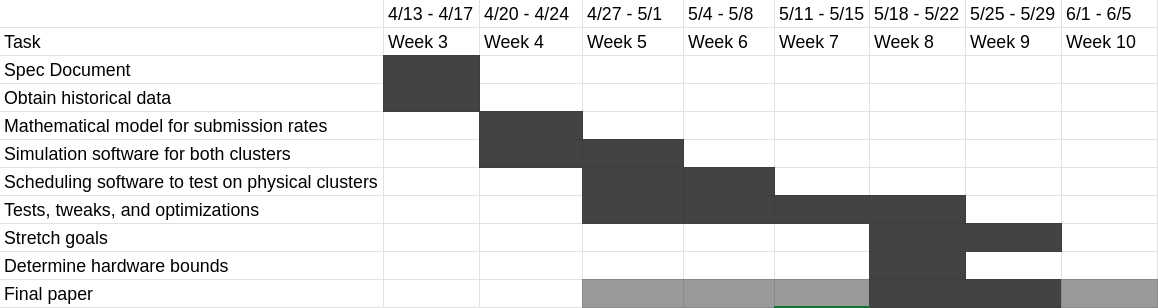
\includegraphics[scale=0.35]{images/timeline.png}
  \caption{Project schedule and timeline, organized by milestone week from project inception through final deliverables.}
\end{figure}

\newpage
\section{Milestones and Schedule}

{\small

\noindent\textbf{Priority Key:} \textbf{P0} = Critical \quad \textbf{P1} = Important \quad \textbf{P2} = Stretch Goal

\vspace{1em}

\begin{itemize}[leftmargin=0pt, itemindent=0pt, labelsep=0pt, label={}]
\item \textbf{M1: Historical Data Collection} \hfill \textit{due Apr 19} \textbf{[P0]}\\
\textit{Lead: Tom (FERPA access required)} \\
Obtain and anonymize student submission logs from CSE 160 WI26. Research cluster simulation approaches and scheduling literature.\\
\textit{Done when: anonymized dataset is ready for modeling and at least two scheduling approaches are identified.}

\item \textbf{M2: Student Submission Model} \hfill \textit{due Apr 26} \textbf{[P0]}\\
\textit{Lead: Abas} \\
Build a Gaussian mixture model (via \texttt{sklearn.mixture}) from historical submission data to capture early-submitter and deadline-submitter behavioral distributions.\\
\textit{Done when: model can generate synthetic submission traces that match observed temporal patterns from WI26.}

\item \textbf{M3: Virtual Simulator} \hfill \textit{due May 3} \textbf{[P0]}\\
\textit{Lead: Ayushmaan} \\
Implement a simulator that ingests synthetic submission traces and distributes tasks to a virtual cluster. Simulator must support variable speed playback and be calibratable to real cluster parameters.\\
\textit{Done when: simulator runs end-to-end on a synthetic workload and produces per-job latency and queue depth metrics.}

\item \textbf{M4: Scheduler Integration \& Virtual Testing} \hfill \textit{due May 10} \textbf{[P0]}\\
\textit{Lead: Richard} \\
Integrate a scheduling policy into the simulator and run weak scaling tests across simulated cluster sizes. Begin generating compute unit estimates for different class sizes.\\
\textit{Done when: weak scaling results are logged and at least one class-size estimate is produced from the virtual cluster.}

\item \textbf{M5: MVP --- Node Count Estimate} \hfill \textit{due May 17} \textbf{[P0]}\\
\textit{Lead: All} \\
Produce a principled estimate of the number of smartphone nodes required to serve a class of $n$ students without meaningful queuing delays, derived from the virtual simulator.\\
\textit{Done when: the capacity model can be queried for an arbitrary class size and returns a justified node allocation with supporting metrics.}

\item \textbf{M6: Physical Cluster Validation} \hfill \textit{due May 24} \textbf{[P2]}\\
\textit{Lead: All (contingent on Qualcomm cluster availability)} \\
Run the scheduling software on physical clusters to validate virtual estimates. Determine hardware bounds and document OOM thresholds.\\
\textit{Done when: at least one class-size estimate from M5 is verified or corrected against real hardware data.}

\item \textbf{M7: Final Paper Draft} \hfill \textit{due May 31} \textbf{[P1]}\\
\textit{Lead: All} \\
Complete a full draft of the final paper incorporating metrics from both virtual and physical runs.\\
\textit{Done when: all sections are written and internal review comments are addressed.}

\item \textbf{M8: Project Web Presence \& Paper Revision} \hfill \textit{due Jun 7} \textbf{[P1]}\\
\textit{Lead: All} \\
Publish project web presence. Incorporate any stretch goal results. Finalize paper.\\
\textit{Done when: web presence is live and paper is submission-ready.}

\item \textbf{Final Submissions:}
    \begin{itemize}
        \item Final Project Video \hfill \textit{due Jun 8}
        \item Final Report \hfill \textit{due Jun 12}
    \end{itemize}
\end{itemize}
}




\newpage

\section*{References}


{
\small

[1] Sherman M., Bassil S., Lipman D., Tuck N., and Martin F. 2013. Impact of auto-grading on an introductory computing course. \textit{Journal of Computing Sciences in Colleges}, 28 (6),
69-75.

[2] Mitra J. 2023. Studying the impact of auto-graders giving immediate feedback in programming assignments. In \textit{Proceedings of the 54th ACM Technical Symposium on Computer Science Education V. 1 (SIGCSE 2023)}. Association for Computing Machinery, New York, NY, USA, 388–394. https://doi.org/10.1145/3545945.3569726

[3] Benotti, L., Aloi, F., Bulgarelli, F.,\ \& Gomez, M. J. (2018). The effect of a web-based coding tool with automatic feedback on students’ performance and perceptions. \textit{‌In Proceedings of the 49th ACM Technical Symposium on Computer Science Education. (SIGCSE 2018)}. 2–7. https://doi.org/10.1145/3159450.3159579

[4] McBroom, J., Jeffries, B., Koprinska, I., \& Yacef, K. (2016). Mining behaviours of students in autograding submission system logs. \textit{International Educational Data Mining Society}.
}

%%%%%%%%%%%%%%%%%%%%%%%%%%%%%%%%%%%%%%%%%%%%%%%%%%%%%%%%%%%%


%%%%%%%%%%%%%%%%%%%%%%%%%%%%%%%%%%%%%%%%%%%%%%%%%%%%%%%%%%%%



\end{document}